%!TEX root = mcmpaper.tex

%===============================模型设计============================================
\section{Problem a model design}
\subsection{The distribution of tourists}
The distribution of passengers into the airport is as followed:
\par
According to the assumption 2, passengers arrive at Poisson flow. The probability of the total number of passengers arriving at the airport in time t is as followed:

% \begin{equation}
% \left.
% \begin{aligned}[b]
%   f(x)=\frac{1}{\sqrt{2\pi }*3.7926}*e^{-\frac{(x-11.2125)^2}{2*14.384}}
% \end{aligned}
% \right.
% \end{equation}

\begin{equation}
\left.
\begin{aligned}[b]
	{P_{n}}(t)=\frac{(\lambda t)^{n}}{n!}*e^{-\lambda t}
\end{aligned}
\right.
\end{equation}

parameter $\lambda$ is the average number of the passengers arrive at unit time. According to 24 hours a day, the total passenger flow is 75000, we calculate out $\lambda$=0.8681 p/s.

\begin{equation}
\left.
\begin{aligned}[b]
	{P_{n}}(t)=\frac{(0.8681t)^{n}}{n!}*e^{-0.8681t}
\end{aligned}
\right.
\end{equation}

the time interval between any two passengers meet the negative exponential distribution $\lambda$=0.8681 p/s, the Distribution function:

\begin{equation}
\left.
\begin{aligned}[b]
	F(t)=1-e^{-0.8681t}~ ~t\geq 0
\end{aligned}
\right.
\end{equation}

Set $R=F(t)$, therefore R is evenly distributed in (0,1). Through inverse transformation we get:

\begin{equation}
\left.
\begin{aligned}
	T=-\frac{1}{0.8681}ln(1-R)=-1.1519ln(1-R)
\end{aligned}
\right.
\end{equation}

Set $U=1-R$,and $U$ is also evenly distributed in $(0,1)$. The time interval $T$ between any two passengers is a random number subject to exponential distribution:

\begin{equation}
\left.
\begin{aligned}
	T=-1.1519ln U
\end{aligned}
\right.
\end{equation}

\subsection{The security process}
According to the assumptions and data offered in the Excel, we can draw a airport security Petri Net Model as followed:

\subsubsection*{Petri Net}
Petri Net is an effective model tool to describe and analyze the system with concurrent and synchronous features. We consider the security check as a system, which is synchronized and concurrent. Using time parameter based on the actual situation to analyze the time of model. Then choose the Generalized Stochastic Petri Net, GSPN to modeling the security check process.

\begin{figure}[H]
\centering
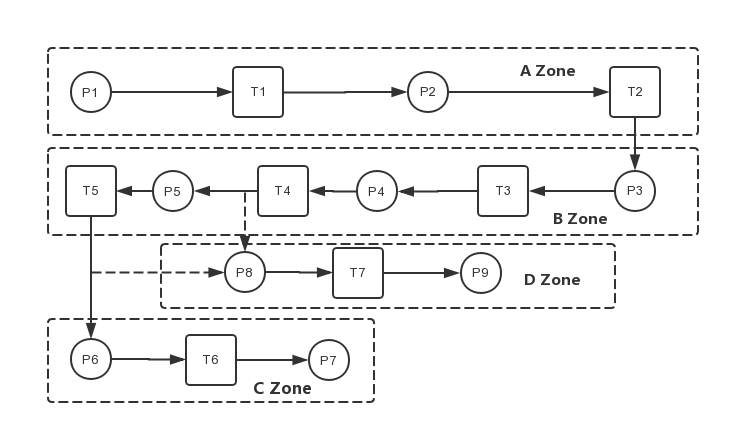
\includegraphics[width=17cm,height=12cm]{/Pic/patrymodel.png}
\caption{Petri network diagram}\label{fig:Petri_Pic}
\end{figure}



\subsubsection*{Symbols in the picture}
\begin{table}[H]
\centering
\caption{Notations}\label{tab:notations}
\begin{tabular}{|c|c|}
\hline
Symbol& Meaning\\
$P_{1}$& Arrivals at the airport \\
\hline
$P_{2}$& Passengers to start receiving identity checks \\\hline
$P_{3}$& Passengers waiting in the queue in Zone B to put their belongings to screening \\\hline
$P_{4}$& Passengers starting to put their belongings on the belt\\\hline
$P_{5}$& Passengers starting to go through scanner\\\hline
$P_{6}$& Passengers packing belongings in Zone C\\\hline
$P_{7}$& Passengers finished the whole process\\\hline
$P_{8}$& Passengers failed step receive a pat-down inspection\\\hline
$P_{9}$& Passengers finished the inspection in Zone D(10\%)
\\\hline
$T_{1}$& Time of waiting for identity verification \\\hline
$T_{2}$& Time of receiving the identity verification(average 11.21s, standard deviation 3.79s) \\\hline
$T_{3}$& Time of waiting for belongings screening\\\hline
$T_{4}$& Time of putting the belongings on the belt\\\hline
$T_{5}$& Time of receiving body inspection(average 41s, standard deviation 6.9s)\\\hline
$T_{6}$& Time of passengers to pack belongings
\\\hline
$T_{7}$& Time of receiving inspection in Zone D
\\\hline

\hline
\end{tabular}
\end{table}


\subsection{Model establishment and solution}
 Based on the above information we can carry out simulation of the airport flow by computer, here are the programming method:
\par
 The entities in the simulation program are composed of passengers, zone A, zone B, zone B and zone D, the controller consists of a time controller and a passenger controller. Here are the description of the relevant attributes and logical description:
\subsubsection*{Attributes Description:}
\paragraph*{Passenger:}
\begin{enumerate}
	\item Time to reach the airport
 	\item Time to leave the security zone
 	\item Whether to buy the  background check
 	\item Time to reach the zone A
 	\item Time to leave the zone A
  	\item Time to reach the zone B
 	\item Time to leave the zone B
 	\item Time to reach the zone C
 	\item Time to leave the zone C
 	\item Time to reach the zone D
 	\item Time to leave the zone D
\end{enumerate}
\paragraph*{Zone}
\begin{enumerate}
	\item Name
	\item The waiting list
\end{enumerate}

\subsubsection*{Logical Description:}
\begin{enumerate}
	\item The time controller increase the time by one second and ask the passenger controller how many passengers reaching the airport at that second. Then the passenger controller put the coming passengers into zone A's waiting list.
	\item The time controller informs all zones to take action
	\item Zone A Reduces the processing time by one for all passengers who are checking documents, then put the passengers who complete the task without problem into zone B's waiting list. Finally, take passengers from zone A's waiting list and set their processing time.
	\item Zone B Reduces the processing time by one for all passengers who are accepting checking, then put the passengers who complete the task without problem into zone C's waiting list and put the other problematic passengers into zone D's waiting list. Finally, take passengers from zone B's waiting list and set their processing time.
	\item Zone C Reduces the processing time by one for all passengers who are packing belongings, then record the data of passengers who complete the task.Finally, delete the passengers and take passengers from zone C's waiting list and set their processing time.
	\item Zone D Reduces the processing time by one for all passengers who are accepting addtional search, then record the data of passengers who complete the task.Finally, delete the passengers and take passengers from zone D's waiting list and set their processing time.
	\item Repeat step 1,2,3,4,5 until all passengers are deleted
	\item Run the script to extract the data and analysis
\end{enumerate}


\subsubsection*{Activity Diagram:}
\begin{figure}[H]
\centering
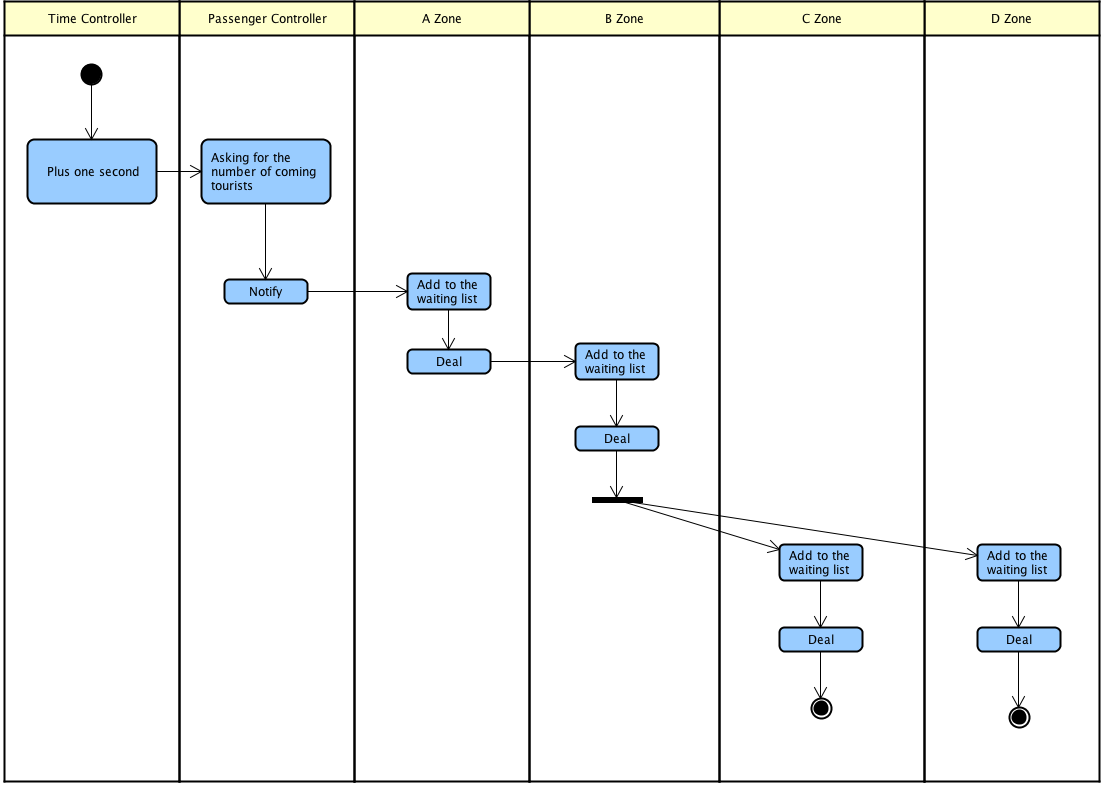
\includegraphics[width=14cm,height=8cm]{/Pic/activity_diagram.png}
\caption{Activity diagram}\label{fig:acd}
\end{figure}

\subsection{Model summary}
According to the above programming ideas for programming simulation, the average time of passengers waiting in each Zone is as followed:

\begin{figure}[H]
\centering
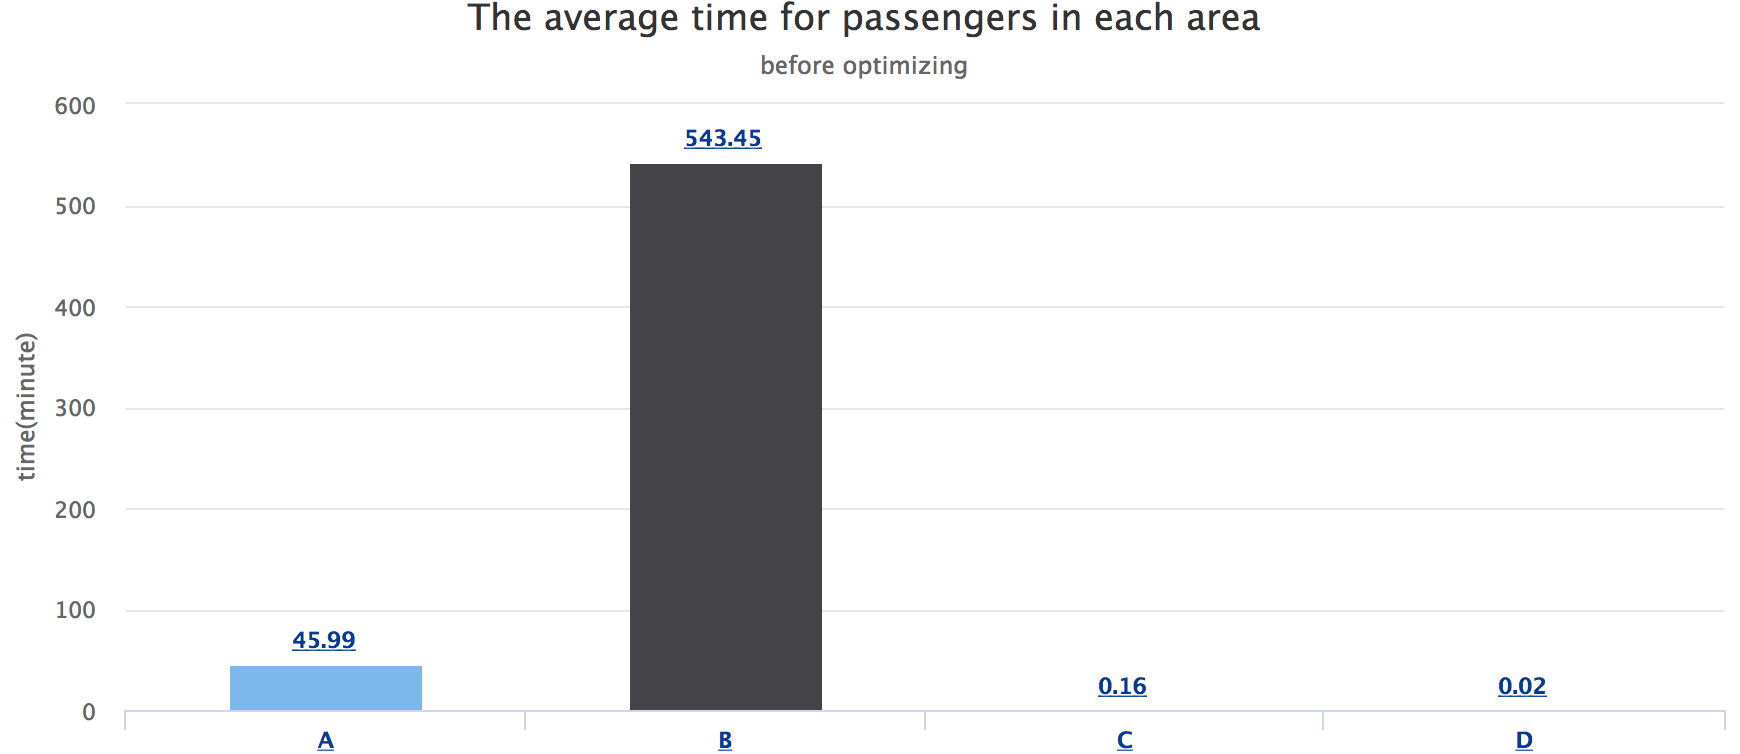
\includegraphics[width=14cm,height=8cm]{/Pic/第一问瓶颈图.png}
\caption{Bottleneck in process}\label{fig:bottleneck}
\end{figure}

We can conclude from the picture that \textbf{the time passengers spent in A and B are the most, which is hundreds times of C and D. So the bottlenecks are Zone A and B, which should be focusing optimized in our future modeling.}








